%%%%%%%%%%%%%%%%%%%%%%%%%%%%%%%%%%%%%%%%%
% Beamer Presentation
% LaTeX Template
% Version 1.0 (10/11/12)
%
% This template has been downloaded from:
% http://www.LaTeXTemplates.com
%
% License:
% CC BY-NC-SA 3.0 (http://creativecommons.org/licenses/by-nc-sa/3.0/)
%
%%%%%%%%%%%%%%%%%%%%%%%%%%%%%%%%%%%%%%%%%

%----------------------------------------------------------------------------------------
%	PACKAGES AND THEMES
%----------------------------------------------------------------------------------------

\documentclass[aspectratio=43,UTF8,10pt,t]{ctexbeamer}

\mode<presentation> {
\usetheme{Madrid}
\setbeamertemplate{footline}[frame number] % To remove the footer line in all slides
\setbeamercolor{page number in head/foot}{fg=blue}
\setbeamertemplate{navigation symbols}{} % To remove the navigation symbols from the bottom of all slides
}

% User Defined Block %%%%%%%%%%%%%%%%%%%%%%%%%%%%%%%%%%%%%%%%%%%%%%%%%%%%%%%%
\usepackage{setspace}
\definecolor{hanblue}{rgb}{0.27, 0.42, 0.81}
\definecolor{indiagreen}{rgb}{0.07, 0.53, 0.03}
\definecolor{indianred}{rgb}{0.8, 0.36, 0.36}
\definecolor{indianyellow}{rgb}{0.89, 0.66, 0.34}
\definecolor{babypink}{rgb}{0.96, 0.76, 0.76}
\definecolor{ao(english)}{rgb}{0.0, 0.5, 0.0}
\setbeamerfont{block title}{size=\normalsize}
\setbeamerfont{block body}{size=\small}
\newenvironment<>{blueblock}[1]{%
  \setbeamercolor{block title}{fg=white,bg=hanblue}%
  \begin{block}#2{#1}}{\end{block}}
\newenvironment<>{greenblock}[1]{%
  \setstretch{1.3}\setbeamercolor{block title}{fg=white,bg=indiagreen}%
  \begin{block}#2{#1}}{\end{block}}
\newenvironment<>{redblock}[1]{%
  \setstretch{1.3}\setbeamercolor{block title}{fg=white,bg=indianred}%
  \begin{block}#2{#1}}{\end{block}}
\newenvironment<>{yellowblock}[1]{%
  \setstretch{1.3}\setbeamercolor{block title}{fg=white,bg=indianyellow}%
  \begin{block}#2{#1}}{\end{block}}

%----------------------------------------------------------------------------------------
%	PACKAGES
%----------------------------------------------------------------------------------------
\usepackage{graphicx} % Allows including images
%\usepackage{tikz}
%\usetikzlibrary{shapes.geometric, arrows}
\usepackage{listings}
\usepackage{multicol}
\lstset{language=C++,
    columns=flexible,
    basicstyle=\footnotesize\ttfamily,                                      % 设定代码字体、大小
    %numbers=left,xleftmargin=2em,framexleftmargin=2em,                   % 在左侧显示行号
    %numberstyle=\color{darkgray},                                        % 设定行号格式
    keywordstyle=\color{blue},                                            % 设定关键字格式
    commentstyle=\color{ao(english)},                                     % 设置代码注释的格式
    stringstyle=\color{brown},                                            % 设置字符串格式
    %showstringspaces=false,                                              % 控制是否显示空格
	%frame=lines,                                                         % 控制外框
    breaklines,                                                           % 控制是否折行
    postbreak=\space,                                                     % 控制折行后显示的标识字符
    breakindent=5pt,                                                      % 控制折行后缩进数量
    emph={size\_t,array,deque,list,map,queue,set,stack,vector,string,pair,tuple}, % 非内置类型
    emphstyle={\color{teal}},
    escapeinside={(*@}{@*)},
}

%----------------------------------------------------------------------------------------
%	TITLE PAGE
%----------------------------------------------------------------------------------------

\title[\textit{C++程序设计:第八章}]{第八章~哈夫编码} % The short title appears at the bottom of every slide, the full title is only on the title page

%\author[李长河]{李长河} % Your name
%\institute[CUG] % Your institution as it will appear on the bottom of every slide, may be shorthand to save space
%{
%中国地质大学(武汉)\\ % Your institution for the title page
%\medskip
%\textit{lichanghe@cug.edu.cn} % Your email address
%}
%\date{} % Date, can be changed to a custom date
\usepackage{indentfirst} 
\parindent=19pt
\begin{document}

%----------------------------------------------------------------------------------------
%	TIKZ FLOWCHART
%----------------------------------------------------------------------------------------
%\tikzstyle{startstop} = [rectangle, rounded corners, minimum width=2cm, minimum height=0.5cm, text centered, draw=black, fill=red!30, font=\tiny]
%\tikzstyle{io} = [trapezium, trapezium left angle=70, trapezium right angle=110, minimum width=0cm, minimum height=0cm, text centered, draw=black, fill=blue!30, font=\tiny]
%\tikzstyle{process} = [rectangle, minimum width=2.5cm, minimum height=1.5cm, text centered, draw=black, fill=orange!30, font=\tiny, text width=2cm]
%\tikzstyle{decision} = [diamond, minimum width=2.5cm, minimum height=2cm, text centered, draw=black, fill=green!30, font=\tiny, text width=1.8cm, aspect=1.1]

\begin{frame}[fragile]{8.6 哈夫曼编码}
\tableofcontents
\end{frame}
\begin{frame}[fragile]{8.6 哈夫曼编码}
\section{引言}
\begin{block}{1 引言}
  哈夫曼(Huffman)编码算法是基于二叉树构建编码压缩结构的,它是数据压缩中经典的一种算法。算法根据文本字符出现的频率(或者权值),重新对字符进行编码。为了缩短编码的长度,我们自然希望频率越高的词,编码越短,这样才能最大化压缩存储文本数据的空间。\\
  假设现在我们要对下面这句歌词“we will we will r u”进行压缩。如果使用ASCII码对这句话编码则为:119 101 32 119 105 108 108 32 119 101 32 119 105 108 108 32 114 32 117(十进制表示)。我们可以看出需要19个字节,也就是至少需要152位的内存空间去存储这些数据。\\
  很显然直接用ASCII码编码很浪费空间,Unicode就更不用说了。下面我们先来统计一下这句话中每个字符出现的频率。如下表,按频率高低已排序:
\\[19pt]
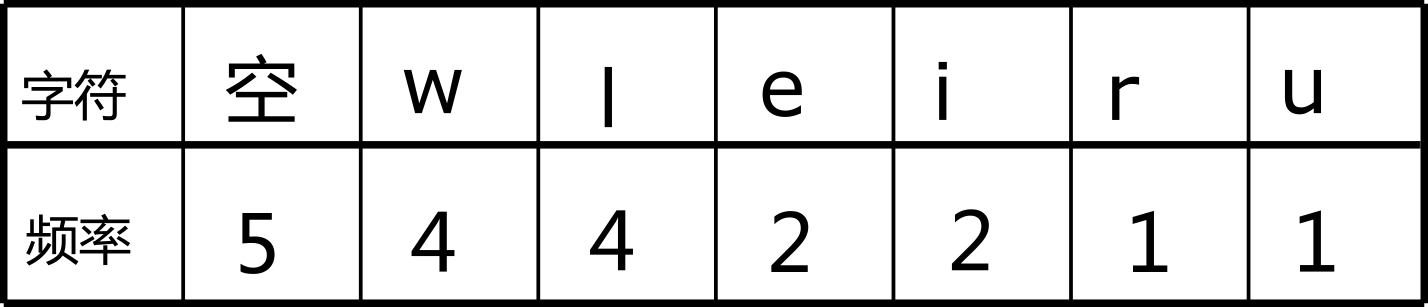
\includegraphics[scale=0.4]{huffman_code_1.png}
\end{block}
\end{frame}

\begin{frame}[fragile]{8.6 哈夫曼编码}
\section{哈夫曼二叉树构建}
\subsection{初始队列}
\begin{block}{2 哈夫曼二叉树构建}
2.1 初始队列\\
  按出现频率高低将其放入一个优先级队列中,从左到右依次为频率逐渐增加。
\\[10pt]
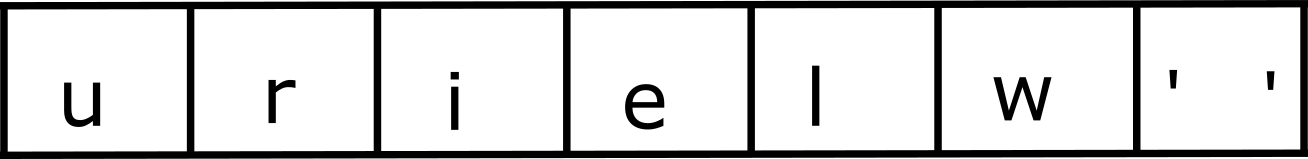
\includegraphics[scale=0.4]{huffman_code_2.png}\\
  将这个队列转换成哈夫曼树,哈夫曼树是一颗带权重的二叉树,权重由队列中每个字符出现的次数(频率)决定。哈夫曼树始终保证权重越大的字符出现在越高的地方。
\subsection{第一步合并}
2.2 第一步合并\\
 从左到右进行合并,依次构建二叉树。第一步取前两个字符u和r来构造初始二叉树,第一个字符作为左节点,第二个元素作为右节点,然后两个元素相加作为新元素,并且两者权重相加作为新元素的权重。
\\[10pt]
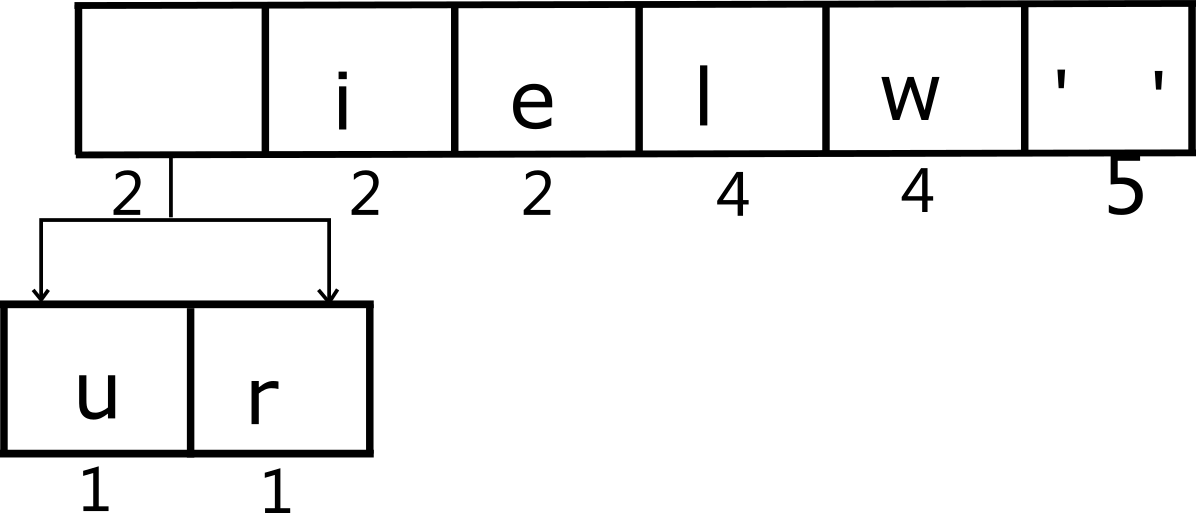
\includegraphics[scale=0.4]{huffman_code_3.png}
\end{block}
\end{frame}


\begin{frame}[fragile]{8.6 哈夫曼编码}
\begin{block}{}
   同理,新元素可以和字符i再合并,如下:
\\[5pt]
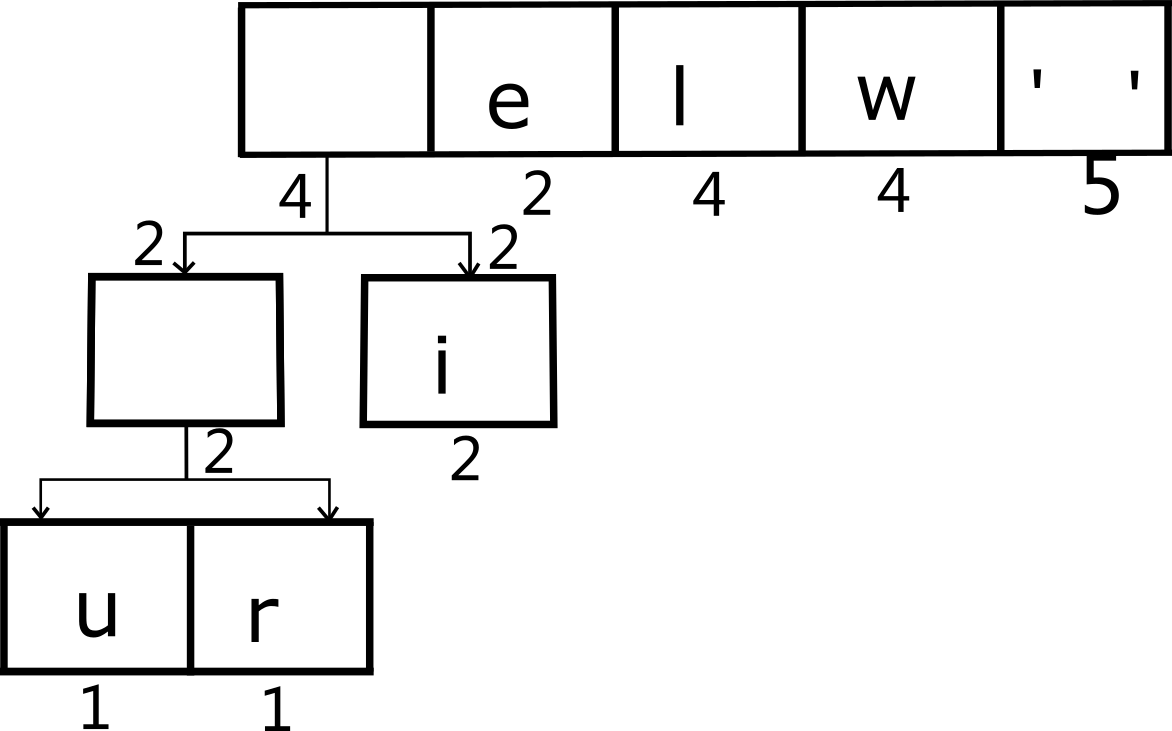
\includegraphics[scale=0.32]{huffman_code_4.png}
\subsection{重新调整队列}\\
2.3 重新调整队列\\
   上图新元素权重相加后结果变大,权重比它前面的权重大,需要对权重进行重新排序。
\\[5pt]
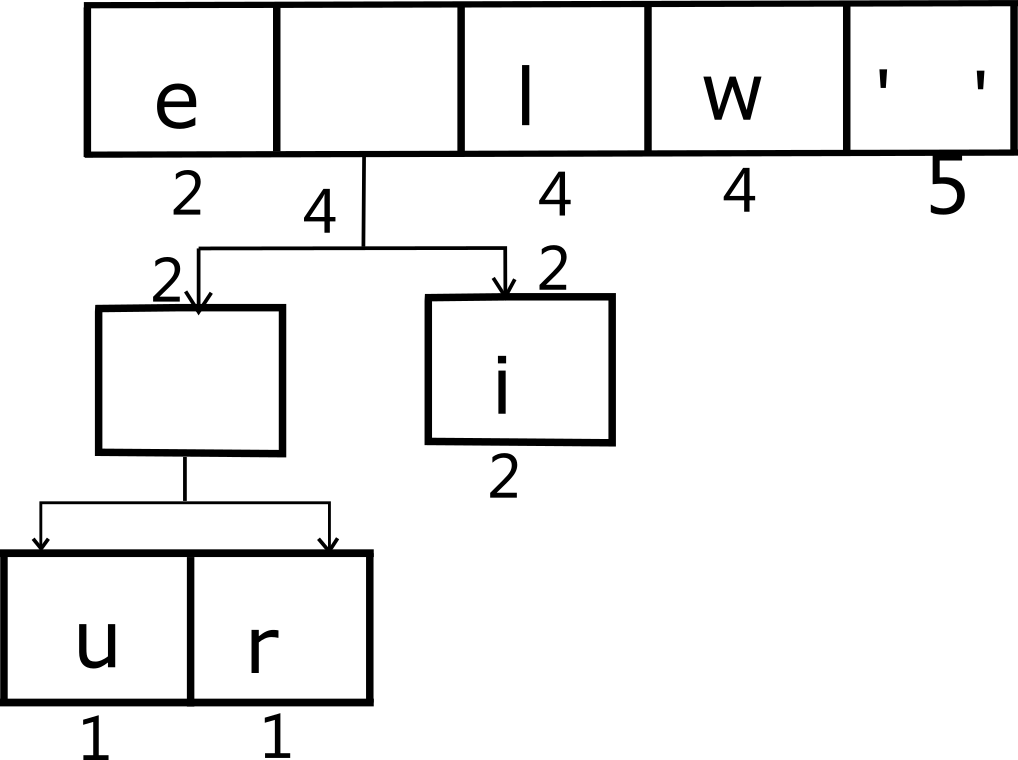
\includegraphics[scale=0.32]{huffman_code_5.png}
\end{block}
\end{frame}


\begin{frame}[fragile]{8.6 哈夫曼编码}
\begin{block}{}
  依次从左到右合并,每合并一次则进行一次队列重新排序调整。如下:
\\[10pt]
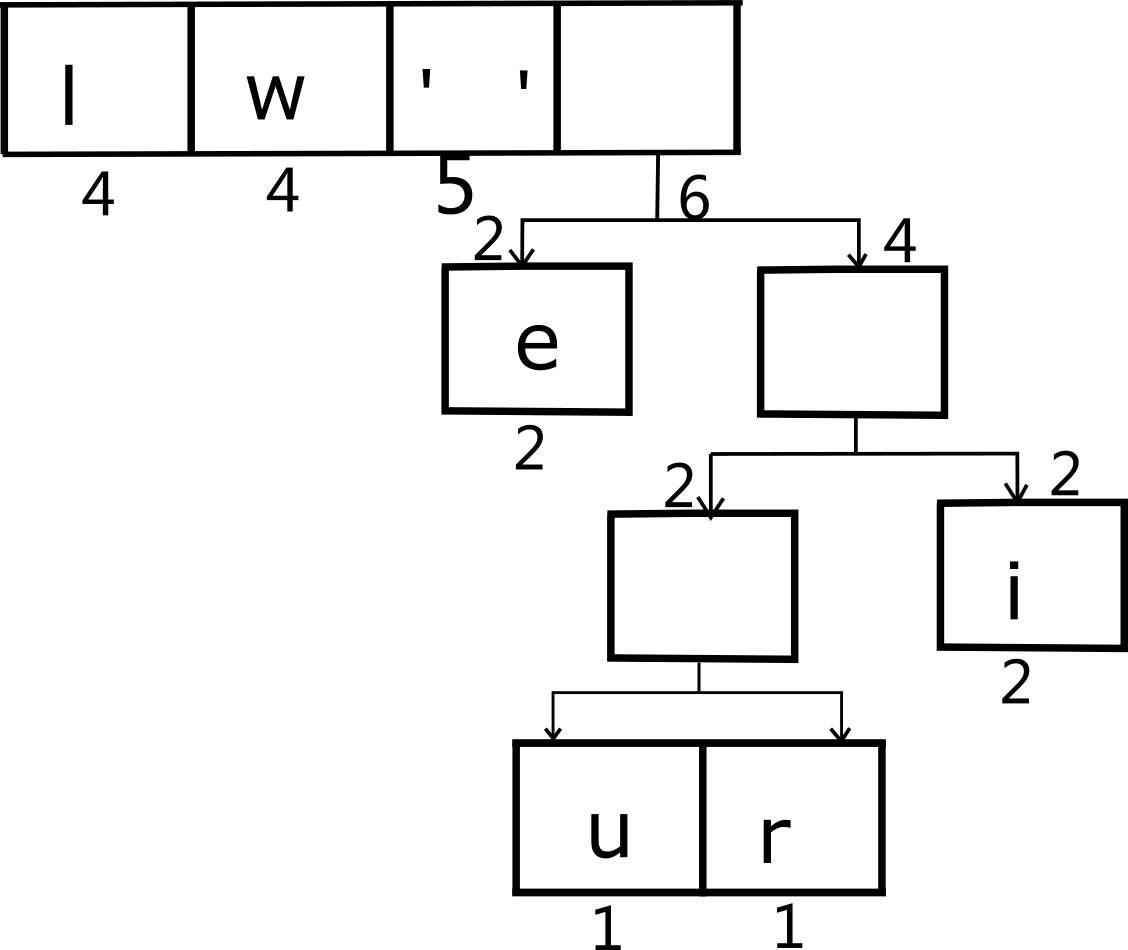
\includegraphics[scale=0.4]{huffman_code_6.png}\\
\end{block}
\end{frame}

\begin{frame}[fragile]{8.6 哈夫曼编码}
\begin{block}{}
   经过多步操作后,得到以下的哈夫曼树,也就是一个带有权重的二叉树:
\\[5pt]
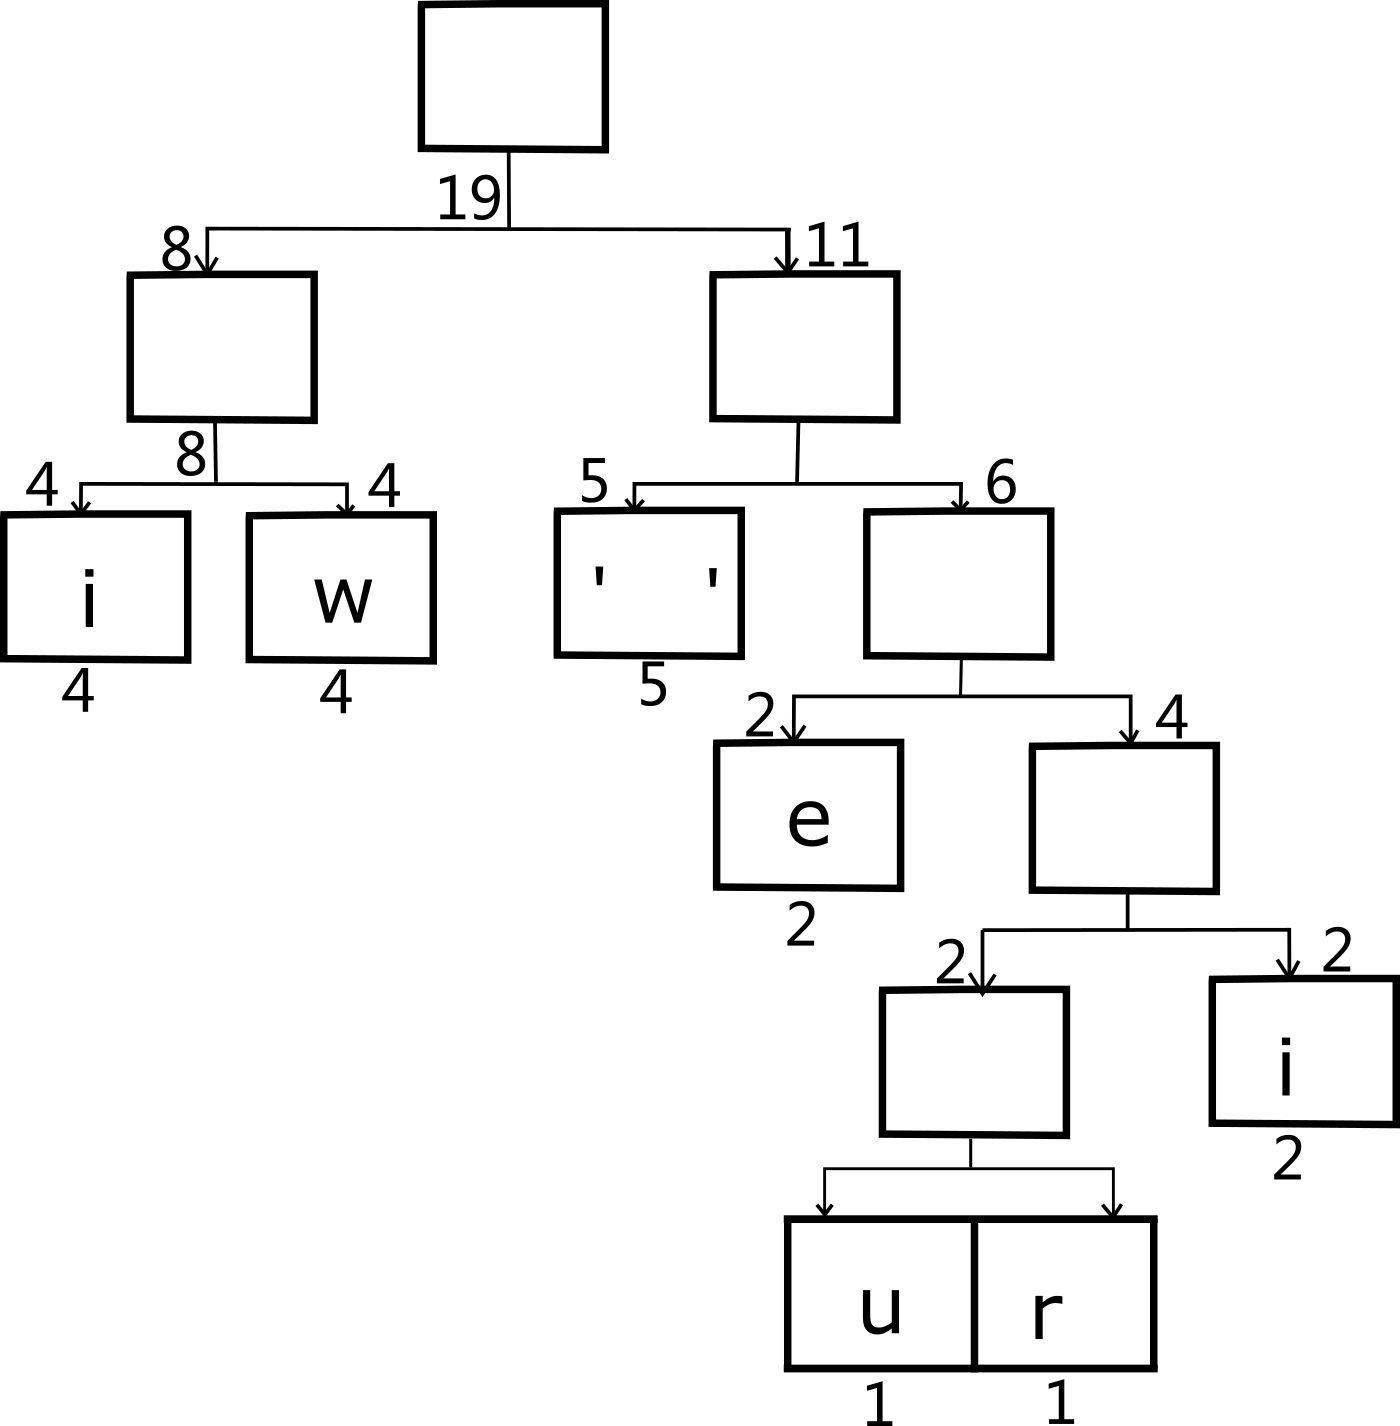
\includegraphics[scale=0.35]{huffman_code_7.png}
\end{block}
\end{frame}

\begin{frame}[fragile]{8.6 哈夫曼编码}
\begin{block}{}
\subsection{哈夫曼编码}
2.4 哈夫曼编码\\
  根据上面带权重的哈夫曼树,就可以进行编码。设置二叉树分支中左边的支路编码为0,右边分支表示为1,如下图\\
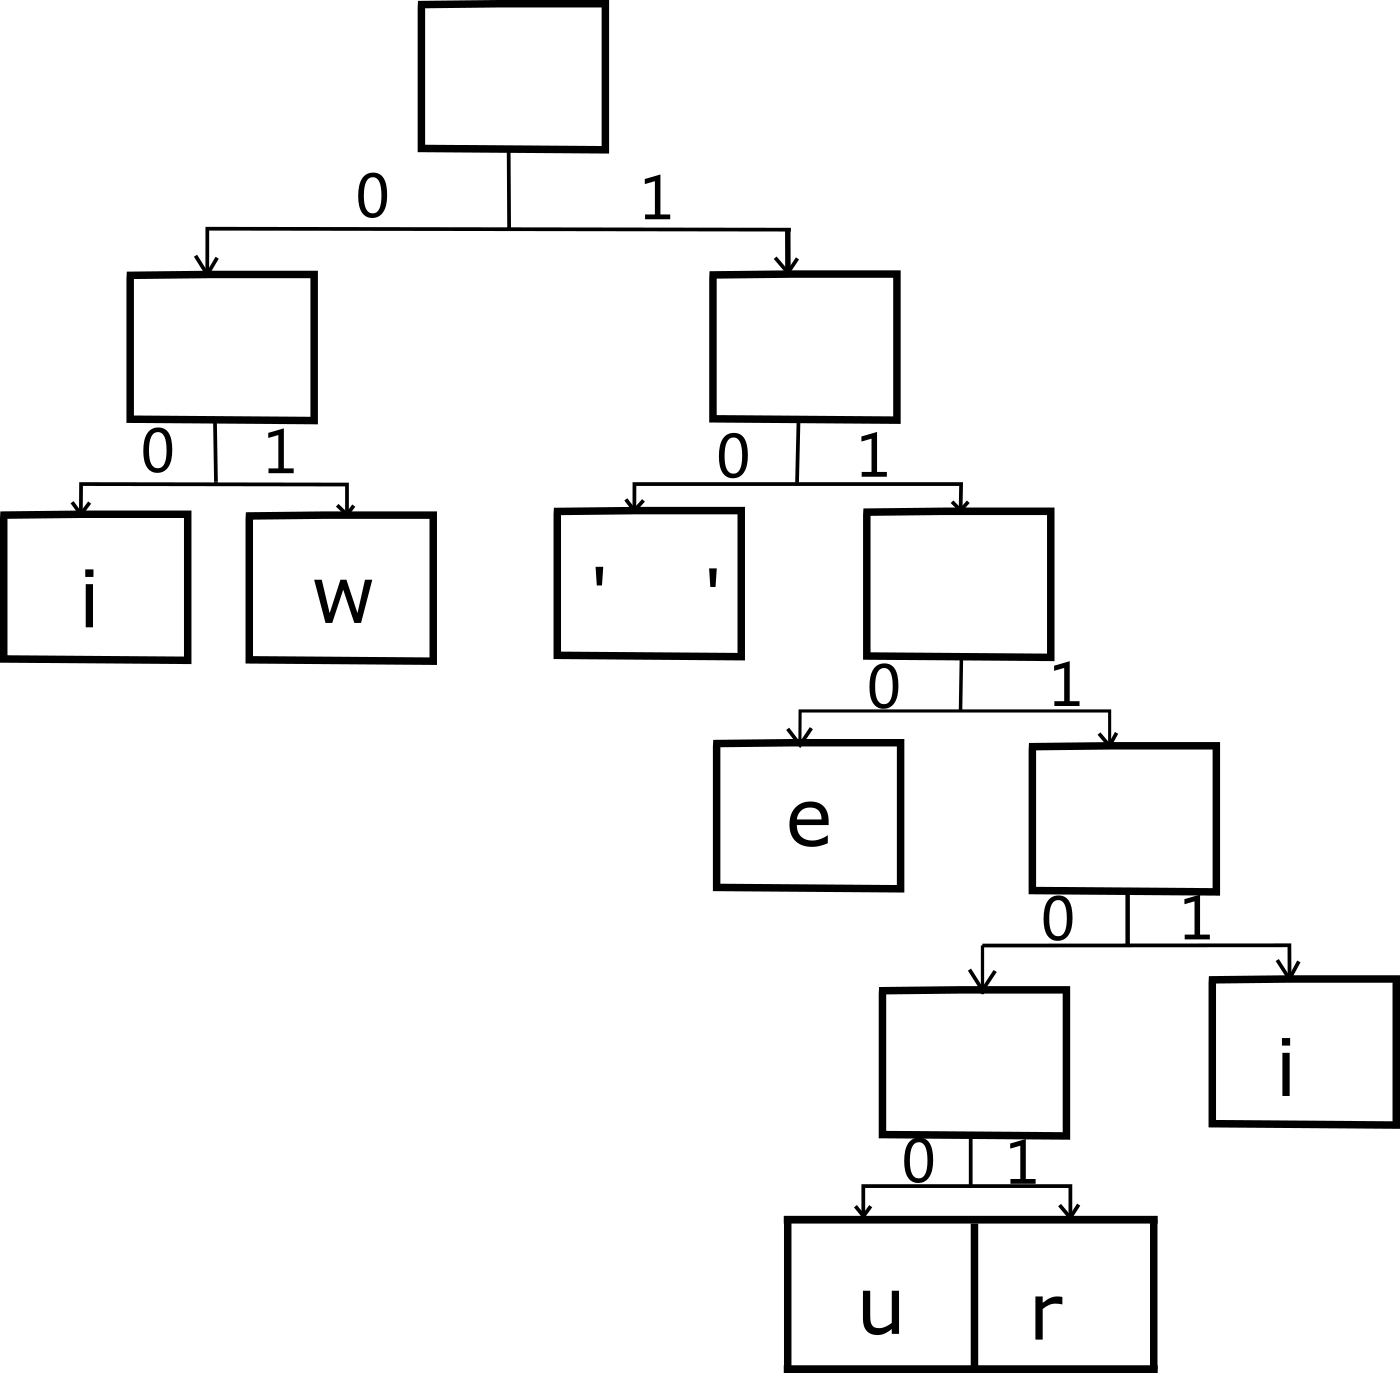
\includegraphics[scale=0.35]{huffman_code_8.png}\\
\end{block}
\end{frame}

\begin{frame}[fragile]{8.6 哈夫曼编码}
\begin{block}{}
  经过这个编码设置之后可以发现,出现频率越高的字符越会在上层,这样它的编码越短;出现频率越低的字符越会在下层,编码较长。经过这样的设计,最终整个文本存储空间才会最大化地缩减。\\
  最终可得到下面的编码表:
\\[5pt]
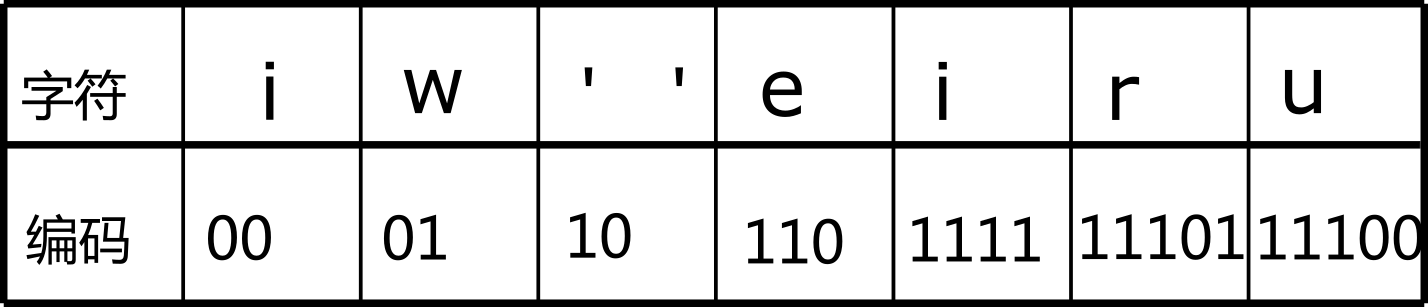
\includegraphics[scale=0.5]{huffman_code_9.png}\\
\subsection{字符串编码}
2.5 字符串编码\\
  有了上面的编码表之后,”we will we will r u”这句进行哈夫曼编码就可以得到很大的压缩,哈夫曼编码表示为:01 110 10 01 1111 00 00 10 01 110 10 01 1111 00 00 10 11101 10 11100。这样最终只需50位内存,比ASCII码编码表示节约了2/3空间,效果很理想。\\
  当然现实中不是简单这样表示的,还需要考虑很多问题。
\end{block}
\end{frame}


\begin{frame}[fragile]{8.6 哈夫曼编码}
\begin{block}{}
\section{补充}
3 补充\\
 哈夫曼树,它是带权路径最小的二叉树,也叫最优二叉树。\\
 它不一定是完全二叉树,也不一定是平衡二叉树,它们描述的完全不是一件事情,完全没有概念上的重叠关系。\\
\subsection{哈夫曼编码练习题}
~\\
~\\
~\\
3.1 哈夫曼编码习题\\
  假设某符号集X中包含7个符号:(s1,s2,s3,s4,s5,s6,s7),它们各自出现的概率分别为:(0.31,0.22,0.18,0.14,0.1,0.04,0.01)。试求集合中各符号的哈夫曼编码?
\end{block}
\end{frame}
\end{document}

